\documentclass[12pt]{article}
\usepackage{geometry}                % See geometry.pdf to learn the layout options. There are lots.
\geometry{letterpaper}                   % ... or a4paper or a5paper or ...
\usepackage{graphicx}
\usepackage{amssymb}
\usepackage{amsthm}
\usepackage{epstopdf}
\usepackage[utf8]{inputenc}
\usepackage[usenames,dvipsnames]{color}
\usepackage[table]{xcolor}
\usepackage{hyperref}
\usepackage{parskip}
\DeclareGraphicsRule{.tif}{png}{.png}{`convert #1 `dirname #1`/`basename #1 .tif`.png}
 
\theoremstyle{definition}
\newtheorem{example}{Example}

\newenvironment{explanation}{%
   \setlength{\parindent}{0pt}
   \itshape
   \color{blue}
}{}

\newenvironment{text}{
}{} 
 
\newcommand{\productname}{Guideo - Audio Guide Platform}
\newcommand{\projectleader}{L. Engleder}
\newcommand{\documentstatus}{  In process }
%\newcommand{\documentstatus}{Submitted}
%\newcommand{\documentstatus}{Released}
\newcommand{\version}{V. 1.9.1}
 
\begin{document}
\begin{titlepage}
\begin{flushright}

\includegraphics[scale=.5]{htlleondinglogo.png}\\
\end{flushright}
 
\vspace{10em}
 
\begin{center}
{\Huge Project Proposal} \\[3em]
{\LARGE \productname} \\[3em]
\end{center}
 
\begin{flushleft}
\begin{tabular}{|l|l|}
\hline
Project Name & \productname \\ \hline
Project Leader & \projectleader \\ \hline
Document state & \documentstatus \\ \hline
Version & \version \\ \hline
\end{tabular}
\end{flushleft}
 
\end{titlepage}
\section*{Revisions}
\begin{tabular}{|l|l|l|}
\hline
\cellcolor[gray]{0.5}\textcolor{white}{Date} & \cellcolor[gray]{0.5}\textcolor{white}{Author} & \cellcolor[gray]{0.5}\textcolor{white}{Change} \\ \hline
September 16, 2019&L. Engleder/P. Quoc/L. Wirth&First version \\ \hline
September 20, 2019&L. Engleder/P. Quoc/L. Wirth& Base information for each section; \\ && proofreading by P. Bauer \\ \hline
September 23, 2019&L. Engleder/P. Quoc/L. Wirth&Minor improvements \\ && and more details;  \\ && proofreading by P. Bauer \\ \hline
September 27, 2019&L. Engleder/P. Quoc/L. Wirth/A. Leeb&writing on planing section \\ \hline
September 29, 2019&L. Engleder/P. Quoc/L. Wirth/A. Leeb&more information in \\ && planning section \\ \hline
September 30, 2019&L. Engleder/P. Quoc/L. Wirth/A. Leeb& improvements on all sections \\ \hline
October 4, 2019&L. Engleder/P. Quoc/L. Wirth/A. Leeb&improvements on all sections\\ \hline
October 7, 2019&L. Engleder/P. Quoc/L. Wirth/A. Leeb&improvements on all sections\\ \hline
October 8, 2019&L. Engleder/P. Quoc/L. Wirth/A. Leeb&graphics and UI description\\ \hline
October 10, 2019&L. Engleder&proof reading and \\ && small adjustments\\ \hline
October 11, 2019&L. Engleder/P. Quoc/L. Wirth/A. Leeb&Milestones\\ \hline

\end{tabular}
\pagebreak
 
\tableofcontents
\pagebreak
 
\section{Introduction}
\begin{text}
Guideo is a platform for users and creators of audio guides. Depending on the location the user can choose from a diverse catalogue of guides, which in turn deliver an informative and highly enjoyable experience. 
It enables anyone to walk through a city or museum without any prior knowledge of it and learn about a variety of subjects such as culture, history, and art. 
Our app not only offers users a unique way to explore a foreign country, but it also opens doors for anyone who wants to express himself through a highly personal, new kind of creative medium. 
 
\end{text}
\pagebreak
 
\section{Initial Situation}
\begin{text}
Currently, there are some ways for people to get information about their traveling destination.\newline

An established, but also somewhat outdated way is to just read about it in a guide book or online.
Buying a generic guide book and reading page to page is a dull task for most people. It takes hours to get into the dry read and it often results in holey knowledge of your travel destination. \newline

And the problem with online travel websites is the huge amount of unfiltered information which distracts from the really exciting things. Moreover, there is no way to enjoy these things in real-time and location-based.\newline
 
Another option for many people is the possibility of hiring a tour guide or joining a bus tour, both promise to offer an educative personalized experience. 
When you consider their high prices many of these tours still happen to have a lot of inconveniences and problems. First of all, there is a huge amount of people who are unable to take part in tours because of hearing impairment or slower walking speed. An important thing to note is also the small pool of languages these services typically offer. Moreover, simply put, it can be a dreadful experience to wander around in an awkward group of strangers you have to endure.\newline
 
For many museums, the installment of an audio guide system can be a big financial burden. Especially the purchase of old outdated hardware for high prices from specialized companies seems out of place in our modern connected world. Keeping these devices functional probably requires a separate technician for maintenance.
Moreover, without regular inspection and cleaning, these systems fail basic hygienic standards. \newline

Although there are archaic audio guides in use in museums there is still no way to enjoy them in a city in general. Our service would provide both locations with fitting guides.
 
\end{text}
 
\pagebreak
 
\section{General Conditions and Constraints}

\subsection{Framework conditions} 
\begin{text}

We are not planning to spend any money except for the cost of a web hosting server. Additional budget points are possible, but not wanted.\newline

As the app was initially and is still imagined as a mobile app. We would develop the app with Angular, a front-end framework, capable of delivering cross-platform mobile solutions. For the server functionality, we will use Java or NodeJS .\newline
 
At the time of writing, only one of our members gathered experiences with Angular, but we are all familiar with the basics.
We also consider ourselves quite confident in our abilities to learn new skills and technologies.\newline
 
We wouldn't cooperate with any other project in our class but if there are museums showing interest in our project we would try to integrate their audio guides
which are already in use. It would greatly expand our catalog of guides and help us establish ourselves in the world of museums.\newline
 
There are no commitments as of now. But we plan to contact some museums and galleries soon.

\end{text}

\subsection{Technical conditions}
\begin{text}

We will develop the app with Angular and the server functionality in combination with IntelliJ.

Versioning will be managed over GitHub.\newline
 
There are currently only our 4 Laptops in use and no Server structure available. And 4 android mobile devices for testing.\newline
 
We will use English when documenting and programming.

\end{text}
  
\pagebreak
 
\section{Project Objectives and System Concepts}
 
\subsection{General}
\begin{text}
In general, we aim to create the same experience you could get in museums with their audio guides, but easily accessible through our app. Normally these guides are only available in museums but our routes will be available at iconic sights, in cities, zoos and much more. All of this at fingertips' reach through our mobile application. 

Further on, the museum and zoos in question will easily be able to provide audio guides to their visitors, completely eliminating the need for expensive equipment and maintenance staff.

They only have to provide the audio files and each location on the map or in the building. Our app will recognize if the user is near a placed audio file and play the desired track.

Not only museums or other institutions can create guides, but every one who is willing to create their own experience is welcomed to upload it to our platform for other users to enjoy. These users can then choose between a variety of audio guides covering different topics and presenting the information in various styles.
\end{text}
 
\subsection{Features}
\begin{text}
The users can listen to audio guides if they are near a specific location. These audio guides will be provided by verified users (e. g. museums, cities, etc.) or the community. Users with popularity among the community and a clean record of guides will be given the option to be promoted to verified status.
When provided and used in a museum the Geo-location based system would be replaced with a tagging system more suited to such an environment.
We are planning on offering different options for museums to install their tagging system. The most modern but also most expensive solution would be the installment of beacons that locate users in small spaces and make the experience fluid and easy.
Another more simple solution would be to tag the stations or artworks with simple numbers combined with QR-codes which are easily scanned and integrated into the experience.\newline
 
To clarify, a guide is a list of different tracks/files each telling a story or giving information about a certain location/object. If a user decides to create a guide he will be given the option to fully create all of its tracks or to build a compilation out of other guides and his files. A guide should be a creative medium encompassing all the stylistic decisions the guide creator made. \newline

But if a listener encounters a location or object he wants to hear about he will be notified and provided with an explanation of another guide. Still, it will not be played automatically, as we think that if a creator decides not to include a location it was a choice he made out of good reasons.
Out of concern that users could miss important locations or that the amount of points in one guide is low, we will offer a Top Track Mode, which automatically plays the most popular track of a specific location.\newline
 
Users that provide audio guides can get verified. Only verified audio guides must be within the regulations and rules. Non-verified audio guides won’t be formally checked but still, need to adhere to the general rules. Users who intentionally provide misinformation, advertise products, etc. will be banned.\newline
 
Users can leave a rating on the audio guides. Inappropriate, faulty or wrong audio guides can be reported by the community. The management of guides will be readily available on the app. A separate website will also provide management features like uploading, updating, and management for museums, creators and the like .\newline

To provide people with recommendations and optimal user experience we plan on collecting some essential data like the languages he or she speaks, preferred language, favorite topics and basic information such as name and email.\newline
 
A notification will pop up if the user is close to a place or point where a verified audio guide is located, but only if the application is running. A pop-up window will appear if the app runs in the foreground. Otherwise, the notification will show up on the status bar and in the notification inbox. 
Non-verified audio guides will only be shown in the Explorer View and will not trigger any kind of notification to reduce the chance of annoying the user.\newline
 
In the Explorer View, the user can explore all available audio guides (verified and non-verified) on a map with the respective locations. Alternatively, there will be a list of audio guides structured around locations (e. g. Linz - Linz Kernzone) with essential information such as language, creator, length of time, topics and popularity. Filtering and Sorting will be enabled.
\end{text}

\subsection{UI and Design}
\begin{text}
When it comes to User Interface we are thinking of separating the app in three major parts that can be accessed through sliding. 
A map view presents the user with a bird's-eye view of his current location. Depending on the mode and state of the user it shows different kind of things and pinpoints different locations. When a user is already listening to a track he will be shown the other locations and the optimal route of the audio guide. 
If he's just browsing he will be shown the main/start locations of verified guides. Through a toggle on the top right he can choose to view the map in best mode and see the most popular guides to the each of the most important locations.

\begin{figure}[ht]
    \caption{Example of the views of our app}
    \centering
    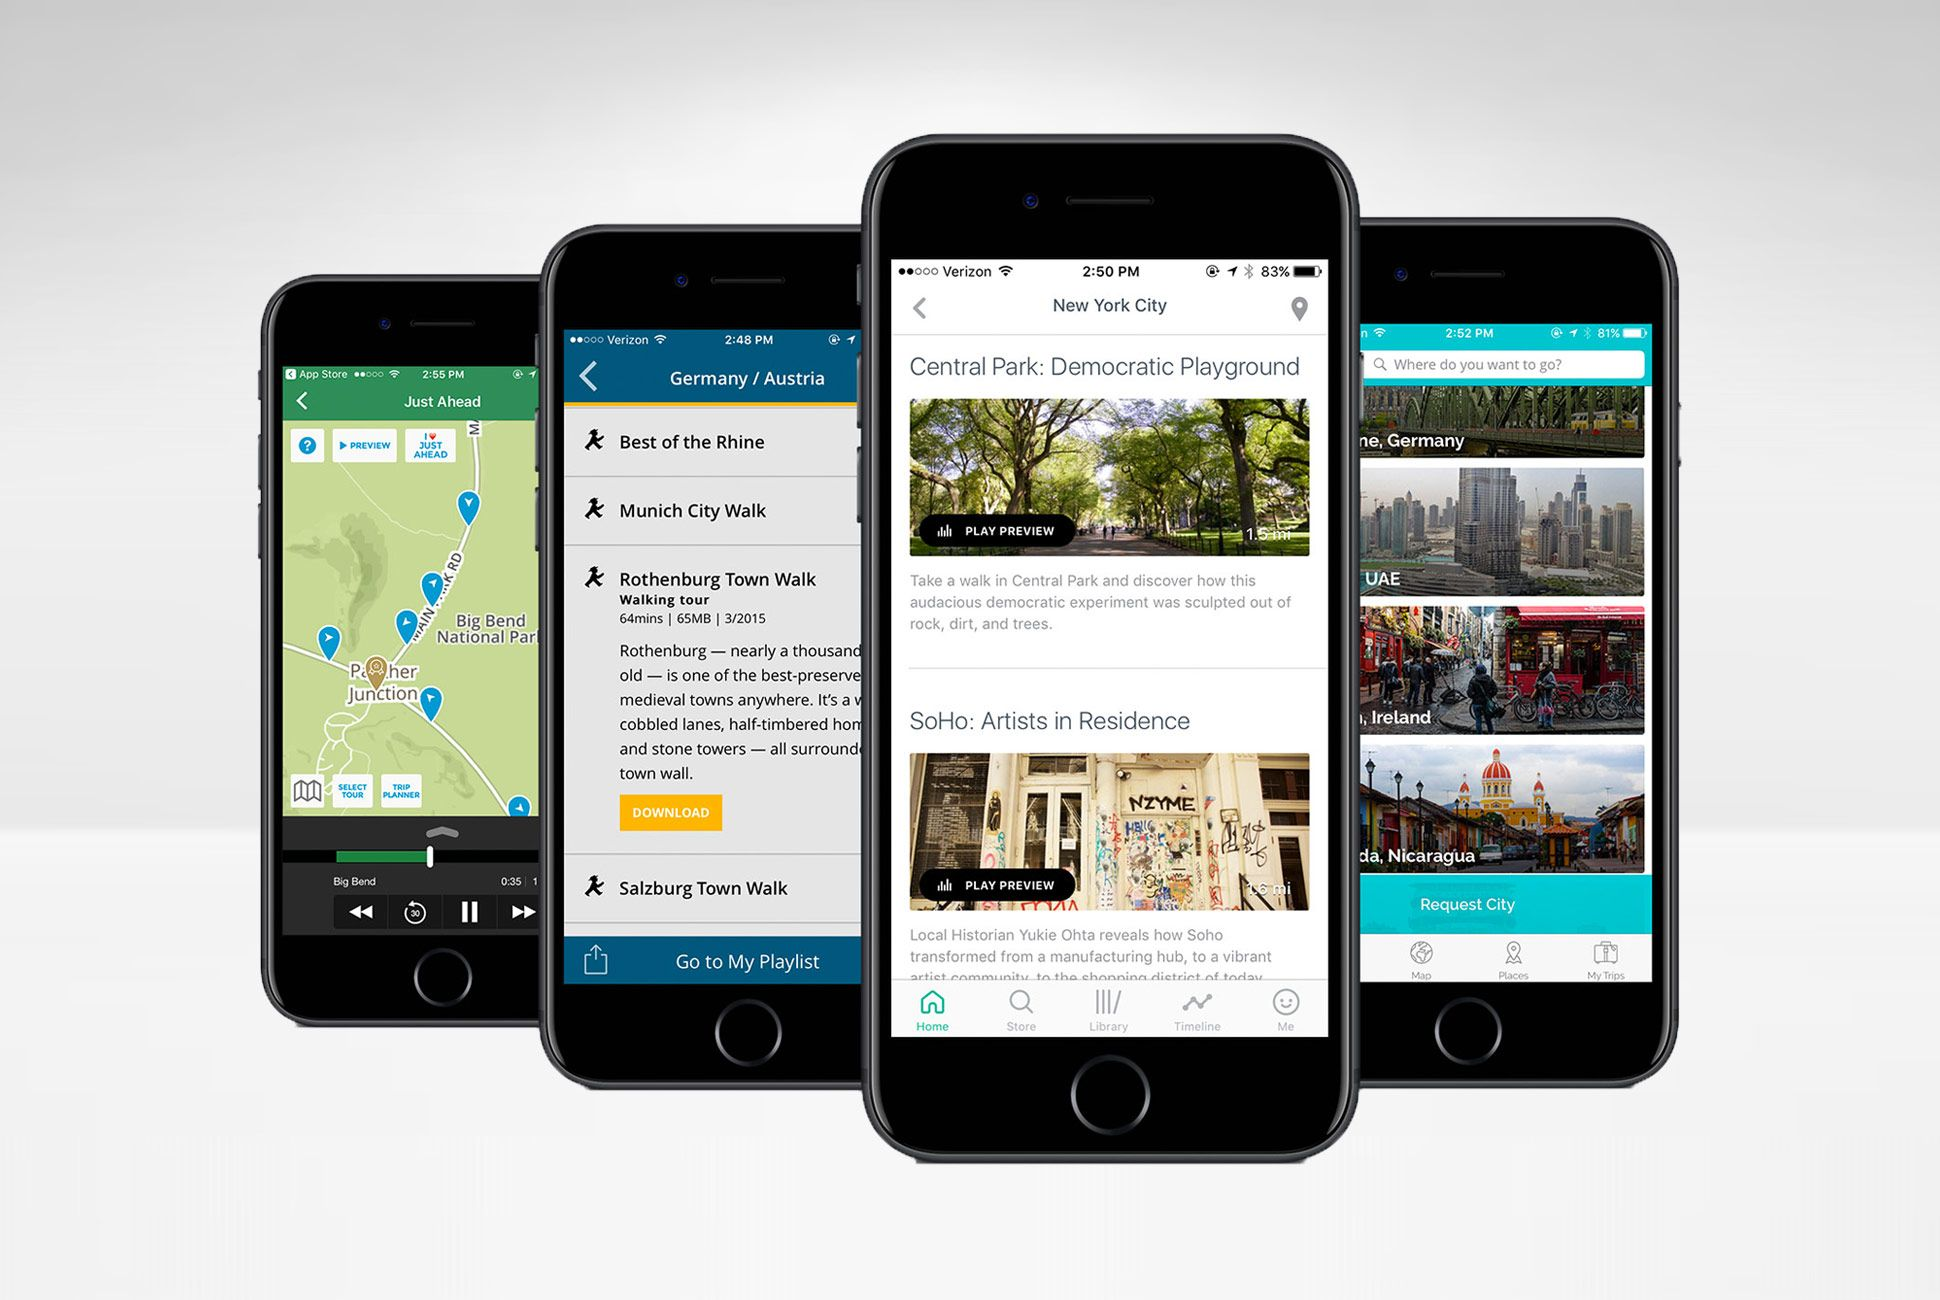
\includegraphics[width=\textwidth]{view_example.jpg}
\end{figure}

Left: Map View with Route Explanation\newline
Middle: Explorer View with Sight on the right
\end{text}

\subsection{Financial}
\begin{text} 
Our aim is that most of the audio guides are cost-free and that our revenue stems from the purchase of audio guides and advertisements.\newline

To financially sustain ourselves we will use a combination of different sources of revenue. We will employ advertisement on free guides at the beginning and end of the tour. This feature will also push users to buy the ad-free application in exchange for money but, this does not mean that all audio guides (like museums, zoos...) on our platform will be provided for free. When selling the guides we will also take a small commission for our services.\newline

Our platform should also provide a payment system to make the purchase of specific audio guides (museums, zoos...) easy and intuitive. 
\end{text}

\subsection{Testing}
\begin{text}
We are planning to test the tagging system in our own school as it shares some features as size and basic architectural structure with a normal museum. It could even be used in events such as ToT to showcase our application and obviously test our systems under more realistic conditions.\newline

Through releasing guides we, our-selves, created, we hope to boost our in app activity and make our product more presentable in the early stages. It enables us to let other people test and try out the first guides.
\end{text}
 
\pagebreak
\section{Opportunities and Risks}
\begin{text}
The project could gain popularity with people who like to travel and at the same time desire a simple way to learn about customs, culture, and history.
Also, cities might be interested in this project to increase tourism due to the popularity of our audio guide catalogue.
It could also turn out successful as a creative platform for creators of this somewhat new medium. We are also exploring the possibility of selling these created guides. The user will be compensated fairly.\newline
 
Another opportunity for expanding the app would be to simulate an audio-visual experience through the use of AR-technology. It could be employed in historical settings and sceneries. Although the idea is very interesting it would require far more development time and expertise in the field.\newline

Opportunities also lie in our current school as it could be used in events such as ToT to showcase our application and test our systems under more realistic conditions.
 
We could face the risk that our catalogue is too small to really consider it as an option.\newline 
 
One of the biggest risks would just be the absence of any traction and popularity among Museums, Zoos and the like. \newline
 
\end{text}
 
\pagebreak
\section{Planning}

\subsection{Milestones}
\begin{itemize}
\large \item Database Structure and Development
\begin{itemize}
    \normalsize
    \item Creating a database in hold of account data, guide information(name, description) and geofences
    \item creating login view in App
    \item create account authentication at the server
    \item \textbf{Finished: 15. November}
\end{itemize}
\item Account Login, Authentication and Management
\begin{itemize}
    \normalsize
    \item creating login view in App
    \item create account authentication at the server
    \item create account management system
    \item \textbf{Finished: 29. November}
\end{itemize}
\item Localization and Notifications
\begin{itemize}
    \normalsize
    \item Geofence initialization and management
    \item Notifications and toggle switch
    \item Geofences in stand-by mode
    \item \textbf{Finished: 20. December}
\end{itemize}
\item Tagging System
\begin{itemize}
    \normalsize
    \item Number Tagging
    \item QR-Code scanning + Selection
    \item \textbf{Finished: 10. January}
    
    \item Beacon Support
\end{itemize}
\item Audio Guide Streaming
\begin{itemize}
    \normalsize
    \item consistent stream 
    \item UI Support for basic functions
    \item automatic playing
    \item \textbf{Finished: 07. February}
\end{itemize}
\item Route Finding
\begin{itemize}
    \normalsize
    \item 
    \item \textbf{ Finished: 28. February }
\end{itemize}
\item Payment System
\begin{itemize}
    \normalsize
    \item Incorporating Payment System into app
    \item Museum Price Settings
    \item \textbf{Finished: ???}
\end{itemize}
\item Guide Creation System (Recording and Tagging)
\begin{itemize}
    \normalsize
    \item file uploading and management
    \item database integration
    \item location - track mapping
    \item geofence settings + best route
    \item \textbf{Finished : 30. June}
\end{itemize} 
\item Archive + Rating + Reporting
\begin{itemize}
    \normalsize
    \item 
    \item \textbf{Finished: ???}
\end{itemize}
\end{itemize}

\subsection{Members}
\begin{tabular}{|l|l|}
\hline
\cellcolor[gray]{0.5}\textcolor{white}{Name} & \cellcolor[gray]{0.5}\textcolor{white}{Role}\\ \hline
Lucas Engleder & Project Leader, Mobile Co-Master and Database Assistant\\ \hline
Patrick Quoc & Mobile Master\\ \hline
Lukas Wirth & Seamodea \\  \hline
Alexander Leeb & Database Master and Server Assistant \\ \hline
\end{tabular}

Role Explanation:
\begin{itemize}
    \item Seamodea
    \begin{itemize}
        \item \textbf{Se}rver
        \item \textbf{A}nd
        \item \textbf{Mo}bile \textbf{De}sign
        \item \textbf{A}rchitect
    \end{itemize} 
\end{itemize}
\subsection{Resources}
\subsubsection{Human Resources}
\begin{text}
Our project is actually a school project which disables us to really consider external programming help, outside of our core team members. We wouldn't use this option anyway as we see this project not only as necessary work, but as an opportunity to learn new things and try innovative technologies.

But regarding design, we are bearing in mind that our capabilities might be limited and in need of an overlooking eye. Possible candidates are colleagues in our school's design branch.\end{text}

\subsubsection{Licenses and Server}
\begin{itemize}
\item License for Jetbrains' IntelliJ Ultimate Edition IDEA to develop Angular Apps.
\item Microsoft's Visual Studio Code and Drifty Co.'s Ionic are under the MIT License.
\item Database License
\end{itemize}

We are considering buying a server if our school isn't able to provide one. In the case of a possible purchase we would need a server with storage capabilities to accommodate our file space needs.

\subsection{Project Management}
\begin{itemize}
    \item Start of project: 18th October 2019
    \item End of project: End of 5th grade
    \newline
    \item First Prototype available: 24th February 2020 (First day of school after semester vacation)
    \item Begin of implementation work: 11th October 2019
    \newline
    \newline
    \item Big blocks of work
    \begin{itemize}
        \item Database and Server Structure
        \item Localization and Notifications
        \item Audio Guide Streaming
        \item Account Login, Authentication and Management
        \item Route Finding and Google maps integration in general
    \end{itemize}
    \item With enough dedication and without major problems in development we estimate it to be hard but quite possible
    \item As already mentioned we will need a server for our application.
    
\end{itemize} 

\end{document}  
